\documentclass[12pt]{report}
\usepackage[utf8x]{inputenc}
\usepackage[dutch]{babel}
\usepackage{amsmath}
\usepackage{graphicx}
\usepackage{listings}
\usepackage{afterpage}
\usepackage[usenames,dvipsnames]{xcolor}
\usepackage{hyperref}
\hypersetup{colorlinks=true, linkbordercolor={0 0 0}, urlcolor=Blue, linkcolor=Black}
\usepackage{amsmath} 
\usepackage{siunitx} 
\usepackage[sc]{mathpazo}
\lstdefinelanguage{VHDL}{
	morekeywords={
		library,use,all,entity,is,port,in,out,end,architecture,of,
		begin,and, if, else
	},
	morecomment=[l]--
}
\lstset{
	numbers=left,
	breaklines=true,
	tabsize=4,
	literate={\ \ }{{\ }}1
}


\usepackage{xcolor}
\colorlet{keyword}{blue!100!black!80}
\colorlet{comment}{green!90!black!90}

\lstdefinestyle{vhdl}{
	language     = VHDL,
	basicstyle   = \ttfamily,
	keywordstyle = \color{keyword}\bfseries,
	commentstyle = \color{comment}
}

\begin{document}
	\begin{titlepage}
		
		\definecolor{landanimal}{cmyk}{1,.60,0,.40}
		\pagecolor{landanimal}\afterpage{\nopagecolor}
		\center	
		
		\color{white}
		\textsc{\LARGE InHolland}\\[1.5cm] % Name of your university/college
		\textsc{\Large VHDL}\\[2.5cm] % Major heading such as course name
		
		
		\huge \bfseries S88-n Protocol in VHDL \\[2.0cm] % Title of your document
		
		\emph{Authors:}\\
		
		\begin{minipage}{0.4\textwidth}
			\begin{flushleft} \large
				
				Koen Groot \\ 549543
			\end{flushleft}
		\end{minipage}
		~
		\begin{minipage}{0.4\textwidth}
			\begin{flushright} \large
				\large Ruben Pera \\ 551198
			\end{flushright}
		\end{minipage}
	
	
		
	\end{titlepage}
\chapter*{Samenvatting}
Dit verslag gaat over een communicatie kunnen opstellen tussen een NI-FPGA bord en een RM88-N schuifregister via het S88 protocol. Dit wordt tot stand gebracht met de hardware beschrijvingstaal VHDL.\\
Ten eerste wordt onderzocht hoe het S88 protocol werkt. Dit blijkt na extensief onderzoek een protocol te zijn om data over een lijn te sturen. Dit wordt verder gebruikt om data heen weer te sturen vanaf het NI-FPGA bord naar het schuifregister. Er wordt gecontroleerd of het werkt door een LED aan te zetten op het NI-FPGA bord.\\\\

Om te kunnen communiceren is echter wel een constant signaal benodigd, het NI-FPGA bord bevat gelukkig een OnBoardClock (ingebouwde klok) waarmee het mogelijk is te controleren wanneer er een signaal wordt opgevangen.\\
De klok werkt echter op 50Mhz terwijl het RM88-N bord slechts 1khz aankan, dus moet de klok eerst naar beneden geschaalt worden.\\\\

In dit verslag wordt dus besproken wat er geprobeerd wordt te behalen en hoe dit behaald wordt. Met in diepte onderzoek naar de middelen gebruikt. Met name de hardware beschrijvings taal VHDL en het S88 timings protocol.
	\tableofcontents
	\clearpage
	
	\chapter{Inleiding}
	[comments]
	Leg in de inleiding van breed naar smal het probleem in zijn context uit.\\
	Je eindigt de inleiding precies daar waar je het probleem globaal beschreven hebt.\\
	Dan in het hoofdstuk specificatie geef je alle onderdelen weer die door fabrikanten aangeleverd worden, voor zover van toepassing. (Let op! Dit is een keuze, vaak is er een wisselwerkng tussen je specificatie en je requirements en daarmee de volgorde van de hoofdstukken.)\\
	Nu komt de probleem stelling met eventuele onderzoeksvragen aan de orde met daarbij de requirements, etc. Een indeling kun je ook op BB vinden. Die is echter niet zaligmakend,\\ aangezien het kan zijn dat het probleem op zich leidt tot onderzoeksvragen die aanleiding geven tot een hardware keuze.\\
	
	Uiteindelijk moet in je verslag een hoofdstuk het logische vervolg zijn op het vorige hoofdstuk.\\
	

	Geef ter illustratie in dit hoofdstuk ook schematische weergaves van de hardware (het NI-FPGA bord en het RM88-N bord).\\
	Hiernaar kun je dan in je tekst verwijzen.
	
	
	
	
	\chapter{Probleem Omschrijving}
\section{Probleem Omschrijving}

De RM88 is ontworpen om een goedkope feedback bus te zijn, de feedback wordt geleverd via het S88 protocol.\\
Het idee is eenvoudig, de RM88 is een serieel schuif register met een parralelle load input, de input zal dus binnenkomen via het timingsprotocol S88.\\
In dit onderzoek gaat er onderzocht worden of dit nagebouwd kan worden met een XILINX Spartan 3E FPGA bord en de harware omschrijf taal VHDL.


\section{Hoofdvraag}
De Hoofdvraag bij dit onderzoek luidt:
\\\\
Hoe kan er op een XILINX Spartan 3E FPGA bord met behulp van de hardware beschrijving taal VHDL een s88 protocol geïmplementeerd worden?
\\

\section{Deelvragen}
Om de Hoofdvraag goed te kunnen beantwoorden zijn er de volgende deelvragen opgesteld:

\begin{enumerate}
	\item Hoe werkt het s88 protocol?
	\item Hoe werkt een XILINX Spartan 3E FPGA bord?
	\item Hoe kan de hardware beschrijving taal VHDL gebruikt worden op het XILINX bord?
	\item Hoe kan een schuifregister aangesloten worden op het XILINX bord?
\end{enumerate}

Pas nadat alle deelvragen beantwoordt zijn kan op de hoofdvraag een volledig antwoord geformuleerd worden.
	\chapter{Specificaties}
	Bij dit project zijn de volgende drie specificaties meegegeven:
	\begin{enumerate}
		\item Ontwerp en imllementeer een test machine voor de S88.
	\end{enumerate}
	\textit{}\chapter{Vereisten}

Om te kunnen onderzoeken of 

De volgende vereisten zijn gesteld aan het te opleveren systeem.

\begin{itemize}
	\item Het XILINX Spartan 3E FPGA bord moet kunnen communiceren met een Field Programmable Gate Array (FPGA).
	\item De communicatie tussen het XILINX bord en de FPGA moet plaatsvinden door middel van het S88 protocol.
	\item De communicatie tussen het XILINX bord en de FPGA wordt als volgt beschreven, het XILINX bord zal via het S88 protocol de eerste byte uit het FPGA lezen.
	\item Het XILINX bord zal geconfigureerd worden met de hardware beschrijving taal VHDL.
\end{itemize}

	\chapter{Analyse}
In dit onderzoek gaat er onderzocht worden of het S88 protocol nagebouwd kan worden met een XILINX Spartan 3E FPGA bord en de harware omschrijf taal VHDL.
\section{deelvragen}
Voor de Analyse zijn er meerdere deelvragen opgesteld,

\begin{enumerate}
	\item Hoe werkt het s88 protocol?
	\item Hoe werkt een XILINX Spartan 3E FPGA bord?
	\item Hoe kan de hardware beschrijving taal VHDL gebruikt worden op het XILINX bord?
	\item Hoe kan een schuifregister aangesloten worden op het XILINX bord?
\end{enumerate}

\subsection{Hoe werkt het s88 protocol?}
Het s88 wordt uitgelegd met behulp van onderstaande afbeelding.
\\\\
Hierin is CENTRALE het in dit project gebruikte XILINX bord. 
\\\\
Een centrale, die hier CENTRALE heet, kan met behulp van het s88 protocol de rechter bus uitlezen. Dit gebeurt met behulp van een schuifregister.
\\\\
Met de DATA OUT poort van de CENTRALE BUS wordt data ingelezen. Deze is verbonden met de Q1 out poort van het schuifregister, hiermee wordt dus informatie van het schuifregister naar de CENTRALE overgedragen.
\\\\
De werking is als volgt, op het moment dat de CENTRALE een positieve flank geeft op de CLOCK en de LATCH hoog is, dan zal het schuifregister de data op Ingang D inlezen. Geeft de CENTRALE een positieve flank en is de LATCH Laag, dan zal het schuifregister één positie opschuiven.
\\\\
Door een puls op RESET te geven worden de buffers gereset en zijn deze weer gereed voor het ontvangen van nieuwe data. 


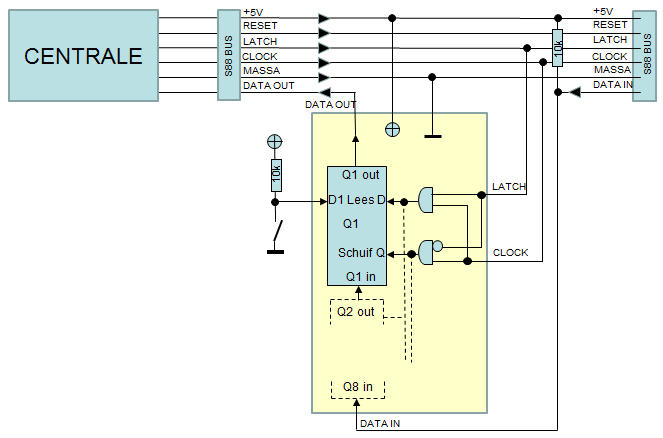
\includegraphics[width=400px]{./img/S88Bus.png}
%http://users.telenet.be/RedDeBist/MBAAN/S88%20terugmelder.htm#S88 bus:
@online{ID,\\
	title = {S88 TERUGMELDERS},\\
	date = {04-03-2016},\\
	url = \url{http://users.telenet.be/RedDeBist/MBAAN/S88\%20terugmelder.htm}
		
	}
\clearpage
	
\subsection{Hoe wordt het XILINX Spartan 3E FPGA bord gebruikt?}
%http://www.xilinx.com/support/documentation/data_sheets/ds312.pdf

\newpage
\subsection{Hoe kan de hardware beschrijving taal VHDL gebruikt worden op het XILINX Spartan 3E FPGA bord?}

%Stuke van Koen

	\chapter{Ontwerp}

Nu alle deel vragen beantwoord zijn in de Analyse kan er verder gegaan worden met het ontwerpen van de werking van het XILINX bord.

\section{Textueel ontwerp van het programma}

De volgende elementen moeten ontworpen en gerealiseerd worden:
\begin{enumerate}
	\item De clock naar beneden schalen zodat de Leds door mensen te zien zijn
	\item De S88 Signalen moeten nagebootst worden
\end{enumerate}

In dit hoofdstuk zal het ontwerpen plaatsvinden, dus in woorden uitgelegd wat er gedaan moet worden, en in het hoofdstuk realiseren wordt het in VHDL gerealiseerd.

\clearpage
\section{Custom Clockrate genereren}

Het eerste wat gedaan moet worden is de clockrate naar beneden schalen, dit wordt gedaan omdat de normale clockrate $\SI{50}{\mega\hertz} $ is.
\\\\
Als een Led met deze frequentie zou knipperen is dat te hoog om met een menselijk oog waar te kunnen nemen, hierom zal de clockrate intern verlaagt moeten worden.
\\\\
Dit zal gebeuren door middel van een interne timer, die iedere clocktick met één verhoogd wordt.
\\\\
Op het moment dat deze timer, die vanaf dit moment TimingCounter genoemt zal worden, een waarde van ${5} \times {10}^5$ bereikt zal er een andere variabele genaamt TijdseenheidCounter met \'e\'en verhoogd worden. 
\\\\
Er zal een Case statement gebruikt worden met als variable de TijdseenheidCounter, en hiermee zal er op elk tijdseenheid de juiste actie uitgevoerd worden.
\clearpage
	\section{De S88 Signalen}

In de Analyze in de sectie "Hoe werkt een s88 protocol" is reeds uitgelegd hoe het s88 protocolr werkt. 
\\
Hier is uit af te leiden dat er door er gebruikt gemaakt wordt van de volgende I/O poorten:

\begin{itemize}
	\item CLOCK
	\item DATA-OUT
	\item LOAD
	\item RESET
\end{itemize}

Het ontwerpen van deze signalen wordt opgesplitst in twee secties, De initialisatie en het daadwerkelijke uitlezen van het schuifregister.

\section{Initialisatie van het schuifregister}


De volgorde van deze signalen wordt beschreven in onderstaande image.
\begin{figure}
	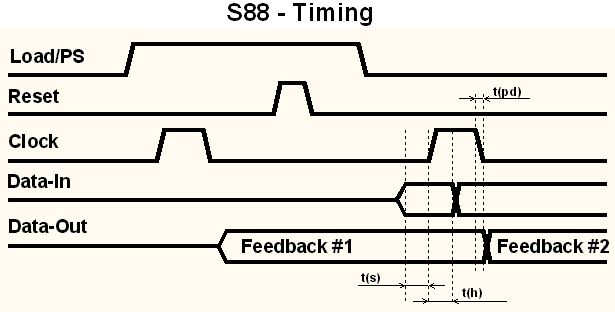
\includegraphics[scale=0.9]{./img/s88timing.png}
	\caption{S88 timing}
\end{figure}


Deze image geeft aan welke poorten wanneer op een logisch 1 gezet moeten worden. Als voorbeeld, de lijn onder Load/PS is de lijn die bij Load hoort. In het begin geeft de lijn een logisch 0 weer, de stijding betekent dat daar de poort op een logisch 1 gezet wordt.
\\\\
Van de poorten Load/PS, Reset en Clock is een UML activiteiten diagram gemaakt, dit is gedaan zodat de volgorde van de signalen overzichtelijker weer te geven is.
\\\\
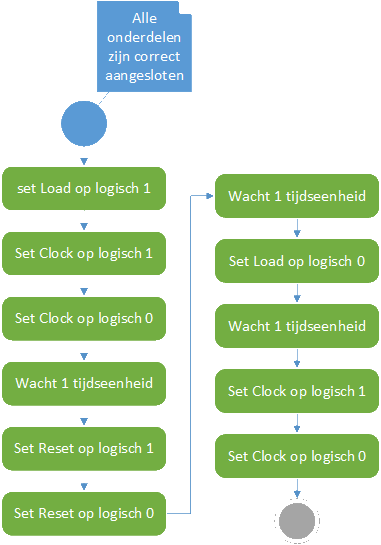
\includegraphics[scale=0.8]{./img/activity.png}
\\\\
Hierin staat één tijdseenheid voor één seconde en is de duur van elke opdracht gelijk aan één tijdseenheid, dus één seconde.\\
Het moet gelezen worden door middel van de pijlen waarin er bovenaan begonnen met lezen wordt bij de blauwe cirkel.\\
Er mag alleen begonnen aan de opdracht als "Alle onderdelen zijn correct aangesloten" waar is, anders heeft het uitvoeren van de in de diagram beschreven opdrachten geen zin.
\\\\
Als er dus gecontroleerd is dat alles correct aangesloten is kan er begonnen worden met de eerste opdracht, in dit geval "Set Load op logisch 1". Nadat deze opdracht uitgevoerd is kan er verdergegaan worden met de opdracht die door middel van de pijl verbonden is, in dit geval "Set Clock op logisch 1". Zo wordt er verdergegaan totdat alle opdracht uitgevoerd zijn, als alle opdrachten uitgevoerd zijn is het schuifregister succesvol geïnitialiseerd.
\newpage
\section{Uitlezen van het Schuifregister}

Nadat de initialisatie voltooid is kan er begonnen worden met het uitlezen van het schuifregister. 
Zoals is beschreven in de analyse kan het schuifregister op de volgende manier uitgelezen worden, er wordt één tijdseenheid een logische 1 op Clock gezet, op de falling-edge van de Clock komt de volgende bit van het schuifregsiter op Data-Out gezet.
\\\\
Dus nadat de Data-Out uitgelezen te hebben kan door middel van de Clock één tijdseenheid een logisch 1 te maken het volgende bit uit het schuifregister op de Data-Out gezet worden. En op die manier kan het hele schuifregister uitgelezen worden.


\begin{flushleft}
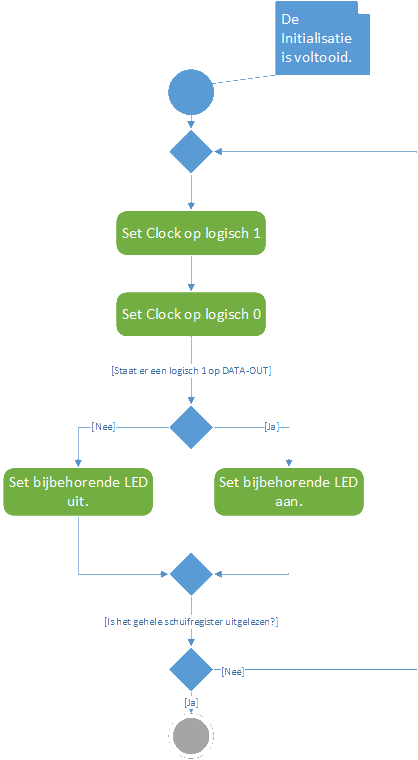
\includegraphics[scale=0.8]{./img/activity2.png}
\end{flushleft}


Wat hier niet goed weergegeven is is dat het net zo vaak uitgevoert zal worden totdat alle bits uit het schuifregister uitgelezen zijn, normaal gesproken wordt dit gedaan met een Loop maar omdat er bij de vereisten al vastgelegd is dat er gebruik gemaakt zal worden van de hardware beschrijving taal VHDL zal dit anders verlopen.\\\\
VHDL beschikt namelijk wel degelijk over een loop maar deze zal hier niet gebruikt worden, de redenatie hierachter is als volgt. Alle elementen worden geclockt op de CustomClock. Een loop kan niet geclockt worden en zal dus zal niet goed kunnen omgaan met de rest van het systeem.
\\\\
Wat er wel gedaan zal worden is het volgende, vanaf het moment dat de initialisatie voltooid is zal er om de tijdseenheid de Clock voor één tijdseenheid logisch 1 gemaakt worden. De tijdseenheid die er dan tussen zit zal gebruikt worden om Data-Out uit te lezen.
Dit zal net zo lang doorgaan totdat alle bits uit het schuifregister door het systeem uitgelezen zijn.
	\chapter{Implementatie}

Voordat er begonnen kan worden wordt er eerst een korte uitleg gegeven over de structuur, syntax en code van de hardware beschrijving taal VHDL.

\section{Hoe wordt VHDL gebruikt}

VHDL begint met een declaratie van alle gebruikte libraries, dit zijn bibliotheken waarin staat hoe de VHDL code met het XILINX bord om moet gaan, bijvoorbeeld waar de aansluitingen zitten.

Na het declareren van de libraries moeten alle IO poorten van het systeem gedeclareerd worden.

Na het declareren van de libraries en de IO poorten kan er nog gebruikt gemaakt worden van interne variabelen, signals genoemt. Waar de IO poorten alleen binair 0 of 1 kunnen zijn kunnen signals meer informatie bevatten, het is mogelijk om integers, bools en dergelijke te gebruiken.

Nadat alles gedeclareerd is kan er begonnen worden met de daadwerkelijke functies.

\clearpage
\section{Declaratie VHDL}

De volgende libraries moeten gedeclareerd worden om de VHDL te kunnen communiceren met het XILINX bord.

\begin{itemize}
	\item ieee;
	\item ieee.std logic 1164.all;
	\item ieee.std logic unsigned.all;
	\item ieee.numeric std.all;
\end{itemize}
\section{Initialisatie van het schuifregister}

Hieronder wordt een lijst gegeven van alle $\boldsymbol{uitgangen}$ die gebruikt gaan worden:
\begin{itemize}
	\item LED0 t/m  LED7.\\
	Deze LEDs worden gebruikt om de toestand van de uit Data-Out ingelezen bits te weer te geven, ofwel 1(Led aan) ofwel 0(led uit).
	\item GPIO16\\
	Dit is de IO poort waarop Load aangesloten wordt.
	\item GPIO17\\
	Dit is de IO poort waarop Reset aangesloten wordt.
	\item GPIO14\\
	Dit is de IO poort waarop Clock aangesloten wordt.

\end{itemize}
In de code zal de naam die ook gebruikt wordt in het tijdschema gebruikt worden, hierdoor is de code beter leesbaar. Er staat bijveerbeeld Load in plaats van GPIO16. \\
\clearpage
Hieronder wordt een lijst gegeven van alle $\boldsymbol{Ingangen}$ die gebruikt gaan worden:
\begin{itemize}
		\item GPIO12\\
		Dit is de IO poort waarop Data-Out aangesloten wordt.
		\item SW0\\
		Dit is de IO poort die aangeeft of de upper of lower byte gelezen wordt.
		\item Onboardclock\\
		Dit is de eerdergenoemde interne clock, deze is geklokt op $\SI{50}{\mega\hertz} $. 
\end{itemize}
In de code zal de naam die ook gebruikt wordt in het tijdschema gebruikt worden, hierdoor is de code beter leesbaar. Er staat bijveerbeeld DataOut in plaats van GPIO12. \\

\section{Uitlezen van het Schuifregister}
Omdat er in totaal twee bytes tegelijk ingelezen kunnen worden met behulp van het schuifregister wordt er een Switch gebruikt om aan te geven welke Byte er uitgelezen moet worden. Hier wordt constant op gecontroleerd bij het uitlezen van de gegevens, deze Zwitch is al genoemd bij de lijst met ingangen.\\\\

Het uitlezen van de registers is een constante herhaling van bijna dezelfde handelingen, deze handelingen bestaan uit het volgende:
\begin{enumerate}
	\item Zet een logische 1 op de Clock.
	\item Zet een logische 0 op de Clock. 
	\item Controleer bij de eerste byte of de Switch een logisch 0 is en bij de tweede byte of de Switch logisch 1 is.
	\item Is dit waar dan kan de bijbehorende LED gelijk gesteld worden aan DataOut.
	Zo niet dan gebeurt er niets.
\end{enumerate}
Hierbij vind nummer één zich plaats op tijd is $x$ en nummer $2$ tot en met $4$ vinden zich plaats op tijd is $x + 1$.\\ 

Er is voor gekozen om dit in een Switch Case opstelling te plaatsen, hierbij wordt het bitpatroon van een variable vergeleken om te achterhalen welke opdracht er uitgevoert moet worden. Dit levert een code op die korter is dan met het gebruik van If statements.\\

De enige veranderingen tussen de verschillende Case statements is:
\begin{enumerate}
	\item Het LED nummer
	\item Of het Lower of Higher Byte geselecteerd is
	\item De index van de Switch
\end{enumerate}

%Hierom is er voor gekozen om dit niet zelf te typen, er is voor gekozen om dit met een Python script te genereren, zie 
	%\chapter{Implementatie}
	%\chapter{Testen}
	%\chapter{Conclusie}
	%\chapter{Bibliografie}
	
\chapter{Apendix}
	\center

\lstinputlisting[style=VHDL]{./code/works.vhd}

			
\end{document}